\documentclass[1p]{elsarticle_modified}
%\bibliographystyle{elsarticle-num}

%\usepackage[colorlinks]{hyperref}
%\usepackage{abbrmath_seonhwa} %\Abb, \Ascr, \Acal ,\Abf, \Afrak
\usepackage{amsfonts}
\usepackage{amssymb}
\usepackage{amsmath}
\usepackage{amsthm}
\usepackage{scalefnt}
\usepackage{amsbsy}
\usepackage{kotex}
\usepackage{caption}
\usepackage{subfig}
\usepackage{color}
\usepackage{graphicx}
\usepackage{xcolor} %% white, black, red, green, blue, cyan, magenta, yellow
\usepackage{float}
\usepackage{setspace}
\usepackage{hyperref}

\usepackage{tikz}
\usetikzlibrary{arrows}

\usepackage{multirow}
\usepackage{array} % fixed length table
\usepackage{hhline}

%%%%%%%%%%%%%%%%%%%%%
\makeatletter
\renewcommand*\env@matrix[1][\arraystretch]{%
	\edef\arraystretch{#1}%
	\hskip -\arraycolsep
	\let\@ifnextchar\new@ifnextchar
	\array{*\c@MaxMatrixCols c}}
\makeatother %https://tex.stackexchange.com/questions/14071/how-can-i-increase-the-line-spacing-in-a-matrix
%%%%%%%%%%%%%%%

\usepackage[normalem]{ulem}

\newcommand{\msout}[1]{\ifmmode\text{\sout{\ensuremath{#1}}}\else\sout{#1}\fi}
%SOURCE: \msout is \stkout macro in https://tex.stackexchange.com/questions/20609/strikeout-in-math-mode

\newcommand{\cancel}[1]{
	\ifmmode
	{\color{red}\msout{#1}}
	\else
	{\color{red}\sout{#1}}
	\fi
}

\newcommand{\add}[1]{
	{\color{blue}\uwave{#1}}
}

\newcommand{\replace}[2]{
	\ifmmode
	{\color{red}\msout{#1}}{\color{blue}\uwave{#2}}
	\else
	{\color{red}\sout{#1}}{\color{blue}\uwave{#2}}
	\fi
}

\newcommand{\Sol}{\mathcal{S}} %segment
\newcommand{\D}{D} %diagram
\newcommand{\A}{\mathcal{A}} %arc


%%%%%%%%%%%%%%%%%%%%%%%%%%%%%5 test

\def\sl{\operatorname{\textup{SL}}(2,\Cbb)}
\def\psl{\operatorname{\textup{PSL}}(2,\Cbb)}
\def\quan{\mkern 1mu \triangleright \mkern 1mu}

\theoremstyle{definition}
\newtheorem{thm}{Theorem}[section]
\newtheorem{prop}[thm]{Proposition}
\newtheorem{lem}[thm]{Lemma}
\newtheorem{ques}[thm]{Question}
\newtheorem{cor}[thm]{Corollary}
\newtheorem{defn}[thm]{Definition}
\newtheorem{exam}[thm]{Example}
\newtheorem{rmk}[thm]{Remark}
\newtheorem{alg}[thm]{Algorithm}

\newcommand{\I}{\sqrt{-1}}
\begin{document}

%\begin{frontmatter}
%
%\title{Boundary parabolic representations of knots up to 8 crossings}
%
%%% Group authors per affiliation:
%\author{Yunhi Cho} 
%\address{Department of Mathematics, University of Seoul, Seoul, Korea}
%\ead{yhcho@uos.ac.kr}
%
%
%\author{Seonhwa Kim} %\fnref{s_kim}}
%\address{Center for Geometry and Physics, Institute for Basic Science, Pohang, 37673, Korea}
%\ead{ryeona17@ibs.re.kr}
%
%\author{Hyuk Kim}
%\address{Department of Mathematical Sciences, Seoul National University, Seoul 08826, Korea}
%\ead{hyukkim@snu.ac.kr}
%
%\author{Seokbeom Yoon}
%\address{Department of Mathematical Sciences, Seoul National University, Seoul, 08826,  Korea}
%\ead{sbyoon15@snu.ac.kr}
%
%\begin{abstract}
%We find all boundary parabolic representation of knots up to 8 crossings.
%
%\end{abstract}
%\begin{keyword}
%    \MSC[2010] 57M25 
%\end{keyword}
%
%\end{frontmatter}

%\linenumbers
%\tableofcontents
%
\newcommand\colored[1]{\textcolor{white}{\rule[-0.35ex]{0.8em}{1.4ex}}\kern-0.8em\color{red} #1}%
%\newcommand\colored[1]{\textcolor{white}{ #1}\kern-2.17ex	\textcolor{white}{ #1}\kern-1.81ex	\textcolor{white}{ #1}\kern-2.15ex\color{red}#1	}

{\Large $\underline{12a_{0916}~(K12a_{0916})}$}

\setlength{\tabcolsep}{10pt}
\renewcommand{\arraystretch}{1.6}
\vspace{1cm}\begin{tabular}{m{100pt}>{\centering\arraybackslash}m{274pt}}
\multirow{5}{120pt}{
	\centering
	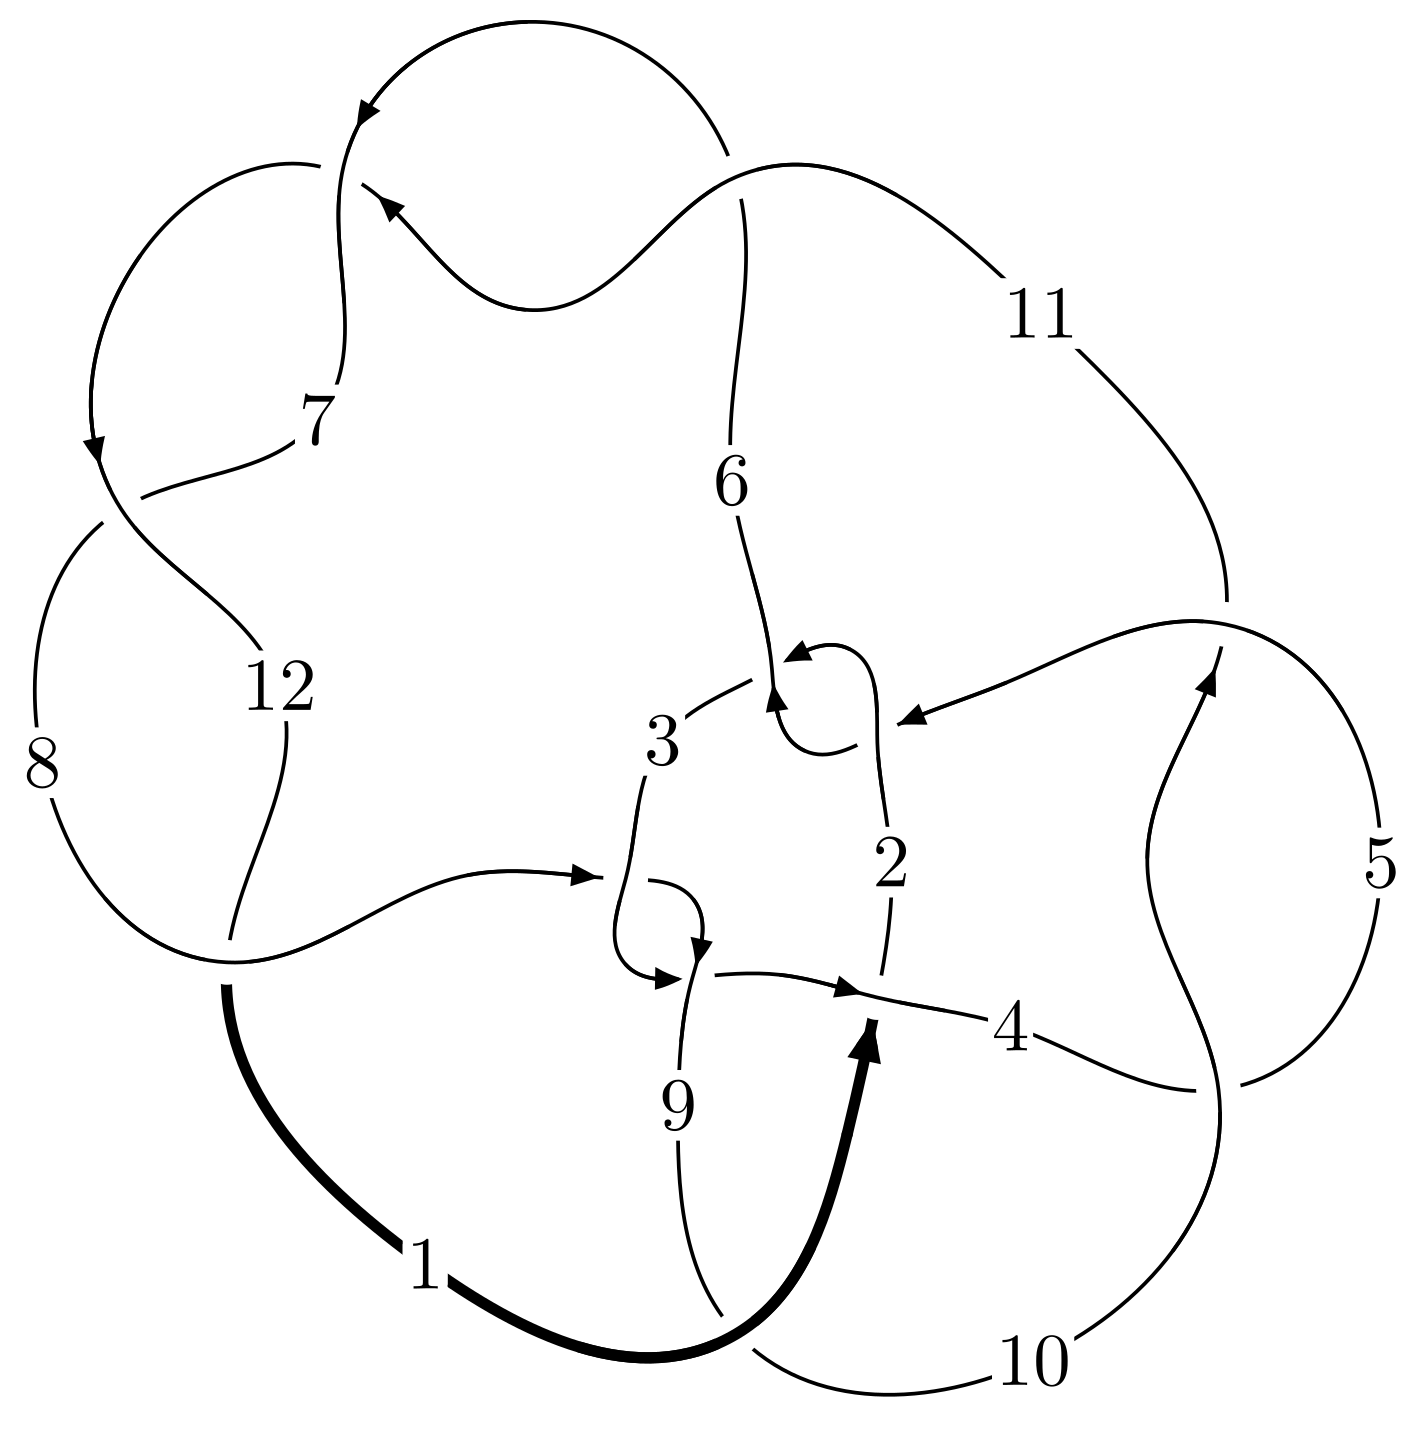
\includegraphics[width=112pt]{../../../GIT/diagram.site/Diagrams/png/1717_12a_0916.png}\\
\ \ \ A knot diagram\footnotemark}&
\allowdisplaybreaks
\textbf{Linearized knot diagam} \\
\cline{2-2}
 &
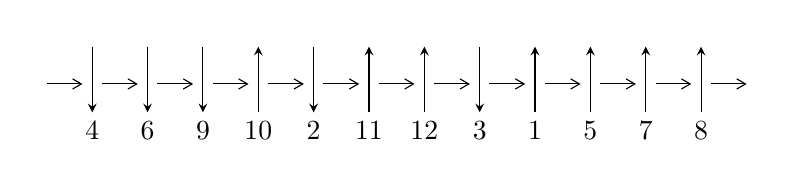
\begin{tikzpicture}[x=20pt, y=17pt]
	% nodes
	\node (C0) at (0, 0) {};
	\node (C1) at (1, 0) {};
	\node (C1U) at (1, +1) {};
	\node (C1D) at (1, -1) {4};

	\node (C2) at (2, 0) {};
	\node (C2U) at (2, +1) {};
	\node (C2D) at (2, -1) {6};

	\node (C3) at (3, 0) {};
	\node (C3U) at (3, +1) {};
	\node (C3D) at (3, -1) {9};

	\node (C4) at (4, 0) {};
	\node (C4U) at (4, +1) {};
	\node (C4D) at (4, -1) {10};

	\node (C5) at (5, 0) {};
	\node (C5U) at (5, +1) {};
	\node (C5D) at (5, -1) {2};

	\node (C6) at (6, 0) {};
	\node (C6U) at (6, +1) {};
	\node (C6D) at (6, -1) {11};

	\node (C7) at (7, 0) {};
	\node (C7U) at (7, +1) {};
	\node (C7D) at (7, -1) {12};

	\node (C8) at (8, 0) {};
	\node (C8U) at (8, +1) {};
	\node (C8D) at (8, -1) {3};

	\node (C9) at (9, 0) {};
	\node (C9U) at (9, +1) {};
	\node (C9D) at (9, -1) {1};

	\node (C10) at (10, 0) {};
	\node (C10U) at (10, +1) {};
	\node (C10D) at (10, -1) {5};

	\node (C11) at (11, 0) {};
	\node (C11U) at (11, +1) {};
	\node (C11D) at (11, -1) {7};

	\node (C12) at (12, 0) {};
	\node (C12U) at (12, +1) {};
	\node (C12D) at (12, -1) {8};
	\node (C13) at (13, 0) {};

	% arrows
	\draw[->,>={angle 60}]
	(C0) edge (C1) (C1) edge (C2) (C2) edge (C3) (C3) edge (C4) (C4) edge (C5) (C5) edge (C6) (C6) edge (C7) (C7) edge (C8) (C8) edge (C9) (C9) edge (C10) (C10) edge (C11) (C11) edge (C12) (C12) edge (C13) ;	\draw[->,>=stealth]
	(C1U) edge (C1D) (C2U) edge (C2D) (C3U) edge (C3D) (C4D) edge (C4U) (C5U) edge (C5D) (C6D) edge (C6U) (C7D) edge (C7U) (C8U) edge (C8D) (C9D) edge (C9U) (C10D) edge (C10U) (C11D) edge (C11U) (C12D) edge (C12U) ;
	\end{tikzpicture} \\
\hhline{~~} \\& 
\textbf{Solving Sequence} \\ \cline{2-2} 
 &
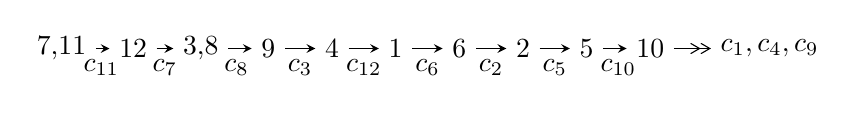
\begin{tikzpicture}[x=23pt, y=7pt]
	% node
	\node (A0) at (-1/8, 0) {7,11};
	\node (A1) at (1, 0) {12};
	\node (A2) at (33/16, 0) {3,8};
	\node (A3) at (25/8, 0) {9};
	\node (A4) at (33/8, 0) {4};
	\node (A5) at (41/8, 0) {1};
	\node (A6) at (49/8, 0) {6};
	\node (A7) at (57/8, 0) {2};
	\node (A8) at (65/8, 0) {5};
	\node (A9) at (73/8, 0) {10};
	\node (C1) at (1/2, -1) {$c_{11}$};
	\node (C2) at (3/2, -1) {$c_{7}$};
	\node (C3) at (21/8, -1) {$c_{8}$};
	\node (C4) at (29/8, -1) {$c_{3}$};
	\node (C5) at (37/8, -1) {$c_{12}$};
	\node (C6) at (45/8, -1) {$c_{6}$};
	\node (C7) at (53/8, -1) {$c_{2}$};
	\node (C8) at (61/8, -1) {$c_{5}$};
	\node (C9) at (69/8, -1) {$c_{10}$};
	\node (A10) at (11, 0) {$c_{1},c_{4},c_{9}$};

	% edge
	\draw[->,>=stealth]	
	(A0) edge (A1) (A1) edge (A2) (A2) edge (A3) (A3) edge (A4) (A4) edge (A5) (A5) edge (A6) (A6) edge (A7) (A7) edge (A8) (A8) edge (A9) ;
	\draw[->>,>={angle 60}]	
	(A9) edge (A10);
\end{tikzpicture} \\ 

\end{tabular} \\

\footnotetext{
The image of knot diagram is generated by the software ``\textbf{Draw programme}" developed by Andrew Bartholomew(\url{http://www.layer8.co.uk/maths/draw/index.htm\#Running-draw}), where we modified some parts for our purpose(\url{https://github.com/CATsTAILs/LinksPainter}).
}\phantom \\ \newline 
\centering \textbf{Ideals for irreducible components\footnotemark of $X_{\text{par}}$} 
 
\begin{align*}
I^u_{1}&=\langle 
-2.91980\times10^{108} u^{81}-4.29606\times10^{108} u^{80}+\cdots+1.92612\times10^{108} b+3.19210\times10^{108},\\
\phantom{I^u_{1}}&\phantom{= \langle  }-5.04794\times10^{108} u^{81}-7.50428\times10^{108} u^{80}+\cdots+1.92612\times10^{108} a-1.67695\times10^{109},\\
\phantom{I^u_{1}}&\phantom{= \langle  }u^{82}+u^{81}+\cdots+10 u-1\rangle \\
I^u_{2}&=\langle 
- u^{12}+8 u^{10}+2 u^9-23 u^8-10 u^7+27 u^6+13 u^5-11 u^4- u^3+4 u^2+b-1,\\
\phantom{I^u_{2}}&\phantom{= \langle  }-2 u^{13}+u^{12}+20 u^{11}-5 u^{10}-80 u^9+u^8+158 u^7+30 u^6-150 u^5-50 u^4+53 u^3+23 u^2+a-4 u-8,\\
\phantom{I^u_{2}}&\phantom{= \langle  }u^{14}-10 u^{12}-2 u^{11}+39 u^{10}+15 u^9-73 u^8-40 u^7+63 u^6+44 u^5-17 u^4-18 u^3-2 u^2+4 u+1\rangle \\
I^u_{3}&=\langle 
u^2+b,\;a-1,\;u^6+u^5-2 u^4-2 u^3-1\rangle \\
I^u_{4}&=\langle 
b+1,\;a-1,\;u-1\rangle \\
I^u_{5}&=\langle 
b+a-1,\;a^2- a-1,\;u-1\rangle \\
\\
\end{align*}
\raggedright * 5 irreducible components of $\dim_{\mathbb{C}}=0$, with total 105 representations.\\
\footnotetext{All coefficients of polynomials are rational numbers. But the coefficients are sometimes approximated in decimal forms when there is not enough margin.}
\newpage
\renewcommand{\arraystretch}{1}
\centering \section*{I. $I^u_{1}= \langle -2.92\times10^{108} u^{81}-4.30\times10^{108} u^{80}+\cdots+1.93\times10^{108} b+3.19\times10^{108},\;-5.05\times10^{108} u^{81}-7.50\times10^{108} u^{80}+\cdots+1.93\times10^{108} a-1.68\times10^{109},\;u^{82}+u^{81}+\cdots+10 u-1 \rangle$}
\flushleft \textbf{(i) Arc colorings}\\
\begin{tabular}{m{7pt} m{180pt} m{7pt} m{180pt} }
\flushright $a_{7}=$&$\begin{pmatrix}0\\u\end{pmatrix}$ \\
\flushright $a_{11}=$&$\begin{pmatrix}1\\0\end{pmatrix}$ \\
\flushright $a_{12}=$&$\begin{pmatrix}1\\- u^2\end{pmatrix}$ \\
\flushright $a_{3}=$&$\begin{pmatrix}2.62078 u^{81}+3.89606 u^{80}+\cdots-39.6810 u+8.70635\\1.51590 u^{81}+2.23043 u^{80}+\cdots-9.19417 u-1.65727\end{pmatrix}$ \\
\flushright $a_{8}=$&$\begin{pmatrix}u\\- u^3+u\end{pmatrix}$ \\
\flushright $a_{9}=$&$\begin{pmatrix}-6.70590 u^{81}-12.1721 u^{80}+\cdots+90.0743 u-10.7546\\2.72204 u^{81}+5.57368 u^{80}+\cdots-61.2733 u+9.72272\end{pmatrix}$ \\
\flushright $a_{4}=$&$\begin{pmatrix}6.65029 u^{81}+6.12344 u^{80}+\cdots-81.0522 u+16.1926\\-3.69683 u^{81}-2.01061 u^{80}+\cdots+53.9722 u-8.26479\end{pmatrix}$ \\
\flushright $a_{1}=$&$\begin{pmatrix}- u^2+1\\u^4-2 u^2\end{pmatrix}$ \\
\flushright $a_{6}=$&$\begin{pmatrix}- u\\u\end{pmatrix}$ \\
\flushright $a_{2}=$&$\begin{pmatrix}3.92048 u^{81}+5.03730 u^{80}+\cdots-55.4423 u+10.6962\\0.216200 u^{81}+1.08919 u^{80}+\cdots+6.56719 u-3.64708\end{pmatrix}$ \\
\flushright $a_{5}=$&$\begin{pmatrix}6.01645 u^{81}+9.73383 u^{80}+\cdots-69.8702 u+4.28812\\-2.02257 u^{81}-2.95608 u^{80}+\cdots+24.6648 u-4.64477\end{pmatrix}$ \\
\flushright $a_{10}=$&$\begin{pmatrix}-7.90580 u^{81}-13.4568 u^{80}+\cdots+100.376 u-9.65178\\3.61742 u^{81}+6.47329 u^{80}+\cdots-70.8432 u+10.9055\end{pmatrix}$\\&\end{tabular}
\flushleft \textbf{(ii) Obstruction class $= -1$}\\~\\
\flushleft \textbf{(iii) Cusp Shapes $= 36.4294 u^{81}+55.9906 u^{80}+\cdots-576.502 u+76.1479$}\\~\\
\newpage\renewcommand{\arraystretch}{1}
\flushleft \textbf{(iv) u-Polynomials at the component}\newline \\
\begin{tabular}{m{50pt}|m{274pt}}
Crossings & \hspace{64pt}u-Polynomials at each crossing \\
\hline $$\begin{aligned}c_{1}\end{aligned}$$&$\begin{aligned}
&u^{82}-3 u^{81}+\cdots+15 u-1
\end{aligned}$\\
\hline $$\begin{aligned}c_{2},c_{5}\end{aligned}$$&$\begin{aligned}
&u^{82}+u^{81}+\cdots-138 u+33
\end{aligned}$\\
\hline $$\begin{aligned}c_{3},c_{8}\end{aligned}$$&$\begin{aligned}
&u^{82}-22 u^{80}+\cdots-4101 u-607
\end{aligned}$\\
\hline $$\begin{aligned}c_{4},c_{10}\end{aligned}$$&$\begin{aligned}
&u^{82}+5 u^{81}+\cdots+112 u-8
\end{aligned}$\\
\hline $$\begin{aligned}c_{6},c_{7},c_{11}\\c_{12}\end{aligned}$$&$\begin{aligned}
&u^{82}+u^{81}+\cdots+10 u-1
\end{aligned}$\\
\hline $$\begin{aligned}c_{9}\end{aligned}$$&$\begin{aligned}
&u^{82}-2 u^{81}+\cdots-24 u+12
\end{aligned}$\\
\hline
\end{tabular}\\~\\
\newpage\renewcommand{\arraystretch}{1}
\flushleft \textbf{(v) Riley Polynomials at the component}\newline \\
\begin{tabular}{m{50pt}|m{274pt}}
Crossings & \hspace{64pt}Riley Polynomials at each crossing \\
\hline $$\begin{aligned}c_{1}\end{aligned}$$&$\begin{aligned}
&y^{82}-13 y^{81}+\cdots-27 y+1
\end{aligned}$\\
\hline $$\begin{aligned}c_{2},c_{5}\end{aligned}$$&$\begin{aligned}
&y^{82}-39 y^{81}+\cdots-42804 y+1089
\end{aligned}$\\
\hline $$\begin{aligned}c_{3},c_{8}\end{aligned}$$&$\begin{aligned}
&y^{82}-44 y^{81}+\cdots-14225097 y+368449
\end{aligned}$\\
\hline $$\begin{aligned}c_{4},c_{10}\end{aligned}$$&$\begin{aligned}
&y^{82}-51 y^{81}+\cdots-13728 y+64
\end{aligned}$\\
\hline $$\begin{aligned}c_{6},c_{7},c_{11}\\c_{12}\end{aligned}$$&$\begin{aligned}
&y^{82}-101 y^{81}+\cdots-110 y+1
\end{aligned}$\\
\hline $$\begin{aligned}c_{9}\end{aligned}$$&$\begin{aligned}
&y^{82}-8 y^{81}+\cdots-216 y+144
\end{aligned}$\\
\hline
\end{tabular}\\~\\
\newpage\flushleft \textbf{(vi) Complex Volumes and Cusp Shapes}
$$\begin{array}{c|c|c}  
\text{Solutions to }I^u_{1}& \I (\text{vol} + \sqrt{-1}CS) & \text{Cusp shape}\\
 \hline 
\begin{aligned}
u &= -0.984782 + 0.188624 I \\
a &= -0.141871 + 0.097301 I \\
b &= -0.334414 + 0.658720 I\end{aligned}
 & \phantom{-}5.90211 - 2.33787 I & \phantom{-0.000000 } 0 \\ \hline\begin{aligned}
u &= -0.984782 - 0.188624 I \\
a &= -0.141871 - 0.097301 I \\
b &= -0.334414 - 0.658720 I\end{aligned}
 & \phantom{-}5.90211 + 2.33787 I & \phantom{-0.000000 } 0 \\ \hline\begin{aligned}
u &= \phantom{-}0.843614 + 0.550628 I \\
a &= \phantom{-}0.787898 + 0.115680 I \\
b &= \phantom{-}0.1163850 - 0.0010731 I\end{aligned}
 & \phantom{-}2.79780 - 0.42396 I & \phantom{-0.000000 } 0 \\ \hline\begin{aligned}
u &= \phantom{-}0.843614 - 0.550628 I \\
a &= \phantom{-}0.787898 - 0.115680 I \\
b &= \phantom{-}0.1163850 + 0.0010731 I\end{aligned}
 & \phantom{-}2.79780 + 0.42396 I & \phantom{-0.000000 } 0 \\ \hline\begin{aligned}
u &= -1.02284\phantom{ +0.000000I} \\
a &= \phantom{-}1.47383\phantom{ +0.000000I} \\
b &= -0.331000\phantom{ +0.000000I}\end{aligned}
 & \phantom{-}0.462297\phantom{ +0.000000I} & \phantom{-0.000000 } 0 \\ \hline\begin{aligned}
u &= -0.783113 + 0.549508 I \\
a &= \phantom{-}0.0588211 + 0.1268950 I \\
b &= -0.86879 - 1.12637 I\end{aligned}
 & -4.73426 - 7.26403 I & \phantom{-0.000000 } 0 \\ \hline\begin{aligned}
u &= -0.783113 - 0.549508 I \\
a &= \phantom{-}0.0588211 - 0.1268950 I \\
b &= -0.86879 + 1.12637 I\end{aligned}
 & -4.73426 + 7.26403 I & \phantom{-0.000000 } 0 \\ \hline\begin{aligned}
u &= \phantom{-}0.887115 + 0.337671 I \\
a &= \phantom{-}0.155583 - 0.193486 I \\
b &= \phantom{-}1.042270 - 0.535647 I\end{aligned}
 & -3.35923 + 0.42248 I & \phantom{-0.000000 } 0 \\ \hline\begin{aligned}
u &= \phantom{-}0.887115 - 0.337671 I \\
a &= \phantom{-}0.155583 + 0.193486 I \\
b &= \phantom{-}1.042270 + 0.535647 I\end{aligned}
 & -3.35923 - 0.42248 I & \phantom{-0.000000 } 0 \\ \hline\begin{aligned}
u &= \phantom{-}0.811426 + 0.677149 I \\
a &= \phantom{-}0.0288692 + 0.0472312 I \\
b &= -0.527577 + 1.199900 I\end{aligned}
 & -0.39025 + 13.28170 I & \phantom{-0.000000 } 0\\
 \hline 
 \end{array}$$\newpage$$\begin{array}{c|c|c}  
\text{Solutions to }I^u_{1}& \I (\text{vol} + \sqrt{-1}CS) & \text{Cusp shape}\\
 \hline 
\begin{aligned}
u &= \phantom{-}0.811426 - 0.677149 I \\
a &= \phantom{-}0.0288692 - 0.0472312 I \\
b &= -0.527577 - 1.199900 I\end{aligned}
 & -0.39025 - 13.28170 I & \phantom{-0.000000 } 0 \\ \hline\begin{aligned}
u &= \phantom{-}0.188934 + 0.907176 I \\
a &= -0.616856 + 0.715162 I \\
b &= -0.157446 + 0.338454 I\end{aligned}
 & -2.29134 - 8.09229 I & \phantom{-0.000000 } 0 \\ \hline\begin{aligned}
u &= \phantom{-}0.188934 - 0.907176 I \\
a &= -0.616856 - 0.715162 I \\
b &= -0.157446 - 0.338454 I\end{aligned}
 & -2.29134 + 8.09229 I & \phantom{-0.000000 } 0 \\ \hline\begin{aligned}
u &= \phantom{-}0.585370 + 0.706438 I \\
a &= \phantom{-}0.0863636 - 0.0965957 I \\
b &= \phantom{-}0.083043 - 1.114300 I\end{aligned}
 & \phantom{-}2.00602 + 4.30322 I & \phantom{-0.000000 } 0 \\ \hline\begin{aligned}
u &= \phantom{-}0.585370 - 0.706438 I \\
a &= \phantom{-}0.0863636 + 0.0965957 I \\
b &= \phantom{-}0.083043 + 1.114300 I\end{aligned}
 & \phantom{-}2.00602 - 4.30322 I & \phantom{-0.000000 } 0 \\ \hline\begin{aligned}
u &= -0.795599 + 0.407080 I \\
a &= -0.817039 + 0.266032 I \\
b &= -0.02769 - 1.43627 I\end{aligned}
 & \phantom{-}3.45231 - 7.58300 I & \phantom{-0.000000 } 0 \\ \hline\begin{aligned}
u &= -0.795599 - 0.407080 I \\
a &= -0.817039 - 0.266032 I \\
b &= -0.02769 + 1.43627 I\end{aligned}
 & \phantom{-}3.45231 + 7.58300 I & \phantom{-0.000000 } 0 \\ \hline\begin{aligned}
u &= \phantom{-}0.770296 + 0.366086 I \\
a &= -1.102450 - 0.449931 I \\
b &= \phantom{-}0.209050 - 0.713360 I\end{aligned}
 & \phantom{-}2.67572 + 6.81110 I & \phantom{-0.000000 } 0 \\ \hline\begin{aligned}
u &= \phantom{-}0.770296 - 0.366086 I \\
a &= -1.102450 + 0.449931 I \\
b &= \phantom{-}0.209050 + 0.713360 I\end{aligned}
 & \phantom{-}2.67572 - 6.81110 I & \phantom{-0.000000 } 0 \\ \hline\begin{aligned}
u &= \phantom{-}1.17627\phantom{ +0.000000I} \\
a &= \phantom{-}0.260420\phantom{ +0.000000I} \\
b &= \phantom{-}0.996259\phantom{ +0.000000I}\end{aligned}
 & -3.39624\phantom{ +0.000000I} & \phantom{-0.000000 } 0\\
 \hline 
 \end{array}$$\newpage$$\begin{array}{c|c|c}  
\text{Solutions to }I^u_{1}& \I (\text{vol} + \sqrt{-1}CS) & \text{Cusp shape}\\
 \hline 
\begin{aligned}
u &= -0.657045 + 0.470711 I \\
a &= -0.122567 + 0.464530 I \\
b &= \phantom{-}0.656971 + 1.206150 I\end{aligned}
 & -2.18416 - 4.72064 I & \phantom{-0.000000 } 0 \\ \hline\begin{aligned}
u &= -0.657045 - 0.470711 I \\
a &= -0.122567 - 0.464530 I \\
b &= \phantom{-}0.656971 - 1.206150 I\end{aligned}
 & -2.18416 + 4.72064 I & \phantom{-0.000000 } 0 \\ \hline\begin{aligned}
u &= \phantom{-}0.695887 + 0.178695 I \\
a &= \phantom{-}0.331121 - 1.049200 I \\
b &= -1.52202 + 1.38533 I\end{aligned}
 & -0.296974 + 0.337709 I & -14.6453 + 19.7980 I \\ \hline\begin{aligned}
u &= \phantom{-}0.695887 - 0.178695 I \\
a &= \phantom{-}0.331121 + 1.049200 I \\
b &= -1.52202 - 1.38533 I\end{aligned}
 & -0.296974 - 0.337709 I & -14.6453 - 19.7980 I \\ \hline\begin{aligned}
u &= -0.561252 + 0.447215 I \\
a &= -0.597055 - 0.069631 I \\
b &= \phantom{-}0.304635 + 0.996919 I\end{aligned}
 & -0.76027 - 3.85816 I & \phantom{-0.000000 -}0. + 6.83350 I \\ \hline\begin{aligned}
u &= -0.561252 - 0.447215 I \\
a &= -0.597055 + 0.069631 I \\
b &= \phantom{-}0.304635 - 0.996919 I\end{aligned}
 & -0.76027 + 3.85816 I & \phantom{-0.000000 } 0. - 6.83350 I \\ \hline\begin{aligned}
u &= -0.126025 + 0.701569 I \\
a &= -0.59662 - 1.32241 I \\
b &= \phantom{-}0.114296 - 0.377897 I\end{aligned}
 & -6.70258 + 3.06709 I & -5.21302 - 2.47341 I \\ \hline\begin{aligned}
u &= -0.126025 - 0.701569 I \\
a &= -0.59662 + 1.32241 I \\
b &= \phantom{-}0.114296 + 0.377897 I\end{aligned}
 & -6.70258 - 3.06709 I & -5.21302 + 2.47341 I \\ \hline\begin{aligned}
u &= -0.236388 + 0.598256 I \\
a &= \phantom{-}0.294774 - 0.609135 I \\
b &= \phantom{-}0.426322 + 1.024910 I\end{aligned}
 & -0.07658 - 4.13532 I & \phantom{-}0.75722 + 4.26107 I \\ \hline\begin{aligned}
u &= -0.236388 - 0.598256 I \\
a &= \phantom{-}0.294774 + 0.609135 I \\
b &= \phantom{-}0.426322 - 1.024910 I\end{aligned}
 & -0.07658 + 4.13532 I & \phantom{-}0.75722 - 4.26107 I\\
 \hline 
 \end{array}$$\newpage$$\begin{array}{c|c|c}  
\text{Solutions to }I^u_{1}& \I (\text{vol} + \sqrt{-1}CS) & \text{Cusp shape}\\
 \hline 
\begin{aligned}
u &= -1.28955 + 0.58878 I \\
a &= -0.0523594 + 0.0124131 I \\
b &= \phantom{-}0.706077 + 0.030045 I\end{aligned}
 & \phantom{-}2.14333 + 2.89478 I & \phantom{-0.000000 } 0 \\ \hline\begin{aligned}
u &= -1.28955 - 0.58878 I \\
a &= -0.0523594 - 0.0124131 I \\
b &= \phantom{-}0.706077 - 0.030045 I\end{aligned}
 & \phantom{-}2.14333 - 2.89478 I & \phantom{-0.000000 } 0 \\ \hline\begin{aligned}
u &= \phantom{-}0.113038 + 0.567992 I \\
a &= -0.569049 - 0.821467 I \\
b &= -0.095569 - 0.935559 I\end{aligned}
 & \phantom{-}0.88681 + 4.41440 I & \phantom{-}3.03410 - 4.57971 I \\ \hline\begin{aligned}
u &= \phantom{-}0.113038 - 0.567992 I \\
a &= -0.569049 + 0.821467 I \\
b &= -0.095569 + 0.935559 I\end{aligned}
 & \phantom{-}0.88681 - 4.41440 I & \phantom{-}3.03410 + 4.57971 I \\ \hline\begin{aligned}
u &= \phantom{-}0.558549 + 0.147764 I \\
a &= \phantom{-}0.621866 + 0.196056 I \\
b &= -0.456183 - 0.414679 I\end{aligned}
 & \phantom{-}0.998059 + 0.188402 I & \phantom{-}10.40306 - 0.95041 I \\ \hline\begin{aligned}
u &= \phantom{-}0.558549 - 0.147764 I \\
a &= \phantom{-}0.621866 - 0.196056 I \\
b &= -0.456183 + 0.414679 I\end{aligned}
 & \phantom{-}0.998059 - 0.188402 I & \phantom{-}10.40306 + 0.95041 I \\ \hline\begin{aligned}
u &= -0.234783 + 0.515407 I \\
a &= \phantom{-}1.32426 + 1.53813 I \\
b &= \phantom{-}0.365229 + 0.093260 I\end{aligned}
 & -3.40619 + 1.28533 I & -2.46945 + 0.12060 I \\ \hline\begin{aligned}
u &= -0.234783 - 0.515407 I \\
a &= \phantom{-}1.32426 - 1.53813 I \\
b &= \phantom{-}0.365229 - 0.093260 I\end{aligned}
 & -3.40619 - 1.28533 I & -2.46945 - 0.12060 I \\ \hline\begin{aligned}
u &= \phantom{-}0.502065 + 0.126289 I \\
a &= -2.39872 - 0.92369 I \\
b &= \phantom{-}0.61945 + 1.69002 I\end{aligned}
 & -0.834967 + 0.544419 I & -9.5439 + 23.8545 I \\ \hline\begin{aligned}
u &= \phantom{-}0.502065 - 0.126289 I \\
a &= -2.39872 + 0.92369 I \\
b &= \phantom{-}0.61945 - 1.69002 I\end{aligned}
 & -0.834967 - 0.544419 I & -9.5439 - 23.8545 I\\
 \hline 
 \end{array}$$\newpage$$\begin{array}{c|c|c}  
\text{Solutions to }I^u_{1}& \I (\text{vol} + \sqrt{-1}CS) & \text{Cusp shape}\\
 \hline 
\begin{aligned}
u &= -0.284642 + 0.381065 I \\
a &= \phantom{-}1.48853 + 0.50264 I \\
b &= \phantom{-}0.008733 - 0.426456 I\end{aligned}
 & -1.50630 + 0.84820 I & -1.82690 - 0.01242 I \\ \hline\begin{aligned}
u &= -0.284642 - 0.381065 I \\
a &= \phantom{-}1.48853 - 0.50264 I \\
b &= \phantom{-}0.008733 + 0.426456 I\end{aligned}
 & -1.50630 - 0.84820 I & -1.82690 + 0.01242 I \\ \hline\begin{aligned}
u &= -1.52579 + 0.01939 I \\
a &= -0.08285 + 2.43592 I \\
b &= -0.54993 - 3.11467 I\end{aligned}
 & \phantom{-}6.46065 - 4.82598 I & \phantom{-0.000000 } 0 \\ \hline\begin{aligned}
u &= -1.52579 - 0.01939 I \\
a &= -0.08285 - 2.43592 I \\
b &= -0.54993 + 3.11467 I\end{aligned}
 & \phantom{-}6.46065 + 4.82598 I & \phantom{-0.000000 } 0 \\ \hline\begin{aligned}
u &= \phantom{-}1.52787 + 0.06405 I \\
a &= \phantom{-}0.02483 - 2.22735 I \\
b &= \phantom{-}0.25321 + 2.46288 I\end{aligned}
 & \phantom{-}5.88122 + 5.76712 I & \phantom{-0.000000 } 0 \\ \hline\begin{aligned}
u &= \phantom{-}1.52787 - 0.06405 I \\
a &= \phantom{-}0.02483 + 2.22735 I \\
b &= \phantom{-}0.25321 - 2.46288 I\end{aligned}
 & \phantom{-}5.88122 - 5.76712 I & \phantom{-0.000000 } 0 \\ \hline\begin{aligned}
u &= \phantom{-}1.54225 + 0.03034 I \\
a &= \phantom{-}0.49740 + 1.73264 I \\
b &= -1.12629 - 2.23338 I\end{aligned}
 & \phantom{-}4.80677 - 0.09764 I & \phantom{-0.000000 } 0 \\ \hline\begin{aligned}
u &= \phantom{-}1.54225 - 0.03034 I \\
a &= \phantom{-}0.49740 - 1.73264 I \\
b &= -1.12629 + 2.23338 I\end{aligned}
 & \phantom{-}4.80677 + 0.09764 I & \phantom{-0.000000 } 0 \\ \hline\begin{aligned}
u &= \phantom{-}0.438034\phantom{ +0.000000I} \\
a &= \phantom{-}4.33297\phantom{ +0.000000I} \\
b &= \phantom{-}0.243064\phantom{ +0.000000I}\end{aligned}
 & -5.42434\phantom{ +0.000000I} & \phantom{-}13.3340\phantom{ +0.000000I} \\ \hline\begin{aligned}
u &= \phantom{-}1.55488 + 0.14908 I \\
a &= -0.15289 - 2.05569 I \\
b &= -0.07056 + 2.52598 I\end{aligned}
 & \phantom{-}6.30459 + 6.05965 I & \phantom{-0.000000 } 0\\
 \hline 
 \end{array}$$\newpage$$\begin{array}{c|c|c}  
\text{Solutions to }I^u_{1}& \I (\text{vol} + \sqrt{-1}CS) & \text{Cusp shape}\\
 \hline 
\begin{aligned}
u &= \phantom{-}1.55488 - 0.14908 I \\
a &= -0.15289 + 2.05569 I \\
b &= -0.07056 - 2.52598 I\end{aligned}
 & \phantom{-}6.30459 - 6.05965 I & \phantom{-0.000000 } 0 \\ \hline\begin{aligned}
u &= -1.56931 + 0.07915 I \\
a &= -0.504205 + 1.215630 I \\
b &= \phantom{-}0.11412 - 1.46849 I\end{aligned}
 & \phantom{-}8.22114 - 1.25008 I & \phantom{-0.000000 } 0 \\ \hline\begin{aligned}
u &= -1.56931 - 0.07915 I \\
a &= -0.504205 - 1.215630 I \\
b &= \phantom{-}0.11412 + 1.46849 I\end{aligned}
 & \phantom{-}8.22114 + 1.25008 I & \phantom{-0.000000 } 0 \\ \hline\begin{aligned}
u &= -1.57829 + 0.02432 I \\
a &= \phantom{-}0.83255 - 2.02283 I \\
b &= -0.10047 + 2.25438 I\end{aligned}
 & \phantom{-}6.44108 - 1.01444 I & \phantom{-0.000000 } 0 \\ \hline\begin{aligned}
u &= -1.57829 - 0.02432 I \\
a &= \phantom{-}0.83255 + 2.02283 I \\
b &= -0.10047 - 2.25438 I\end{aligned}
 & \phantom{-}6.44108 + 1.01444 I & \phantom{-0.000000 } 0 \\ \hline\begin{aligned}
u &= \phantom{-}1.59304 + 0.13349 I \\
a &= \phantom{-}0.48960 - 2.30928 I \\
b &= -1.09569 + 3.07315 I\end{aligned}
 & \phantom{-}5.44937 + 6.93869 I & \phantom{-0.000000 } 0 \\ \hline\begin{aligned}
u &= \phantom{-}1.59304 - 0.13349 I \\
a &= \phantom{-}0.48960 + 2.30928 I \\
b &= -1.09569 - 3.07315 I\end{aligned}
 & \phantom{-}5.44937 - 6.93869 I & \phantom{-0.000000 } 0 \\ \hline\begin{aligned}
u &= -1.61613 + 0.05731 I \\
a &= -0.86864 - 2.17772 I \\
b &= \phantom{-}1.34031 + 2.38505 I\end{aligned}
 & \phantom{-}7.71340 - 1.27145 I & \phantom{-0.000000 } 0 \\ \hline\begin{aligned}
u &= -1.61613 - 0.05731 I \\
a &= -0.86864 + 2.17772 I \\
b &= \phantom{-}1.34031 - 2.38505 I\end{aligned}
 & \phantom{-}7.71340 + 1.27145 I & \phantom{-0.000000 } 0 \\ \hline\begin{aligned}
u &= -1.60197 + 0.23933 I \\
a &= -0.21626 + 1.64990 I \\
b &= -0.42879 - 2.17532 I\end{aligned}
 & \phantom{-}9.34734 - 7.89119 I & \phantom{-0.000000 } 0\\
 \hline 
 \end{array}$$\newpage$$\begin{array}{c|c|c}  
\text{Solutions to }I^u_{1}& \I (\text{vol} + \sqrt{-1}CS) & \text{Cusp shape}\\
 \hline 
\begin{aligned}
u &= -1.60197 - 0.23933 I \\
a &= -0.21626 - 1.64990 I \\
b &= -0.42879 + 2.17532 I\end{aligned}
 & \phantom{-}9.34734 + 7.89119 I & \phantom{-0.000000 } 0 \\ \hline\begin{aligned}
u &= -1.62865 + 0.10885 I \\
a &= -0.27752 + 1.88885 I \\
b &= \phantom{-}0.60651 - 2.82092 I\end{aligned}
 & \phantom{-}10.91440 - 8.63897 I & \phantom{-0.000000 } 0 \\ \hline\begin{aligned}
u &= -1.62865 - 0.10885 I \\
a &= -0.27752 - 1.88885 I \\
b &= \phantom{-}0.60651 + 2.82092 I\end{aligned}
 & \phantom{-}10.91440 + 8.63897 I & \phantom{-0.000000 } 0 \\ \hline\begin{aligned}
u &= \phantom{-}1.63599 + 0.11853 I \\
a &= \phantom{-}0.13839 + 1.88321 I \\
b &= \phantom{-}0.63901 - 2.35405 I\end{aligned}
 & \phantom{-}11.7947 + 9.5991 I & \phantom{-0.000000 } 0 \\ \hline\begin{aligned}
u &= \phantom{-}1.63599 - 0.11853 I \\
a &= \phantom{-}0.13839 - 1.88321 I \\
b &= \phantom{-}0.63901 + 2.35405 I\end{aligned}
 & \phantom{-}11.7947 - 9.5991 I & \phantom{-0.000000 } 0 \\ \hline\begin{aligned}
u &= \phantom{-}1.63569 + 0.16394 I \\
a &= -0.60372 + 1.93511 I \\
b &= \phantom{-}1.25447 - 2.32571 I\end{aligned}
 & \phantom{-}3.49190 + 9.98671 I & \phantom{-0.000000 } 0 \\ \hline\begin{aligned}
u &= \phantom{-}1.63569 - 0.16394 I \\
a &= -0.60372 - 1.93511 I \\
b &= \phantom{-}1.25447 + 2.32571 I\end{aligned}
 & \phantom{-}3.49190 - 9.98671 I & \phantom{-0.000000 } 0 \\ \hline\begin{aligned}
u &= -1.64218 + 0.10635 I \\
a &= \phantom{-}1.02828 + 1.40183 I \\
b &= -1.70059 - 1.85899 I\end{aligned}
 & \phantom{-}5.25941 - 2.18573 I & \phantom{-0.000000 } 0 \\ \hline\begin{aligned}
u &= -1.64218 - 0.10635 I \\
a &= \phantom{-}1.02828 - 1.40183 I \\
b &= -1.70059 + 1.85899 I\end{aligned}
 & \phantom{-}5.25941 + 2.18573 I & \phantom{-0.000000 } 0 \\ \hline\begin{aligned}
u &= \phantom{-}1.64631 + 0.13035 I \\
a &= -0.166642 - 1.110980 I \\
b &= -0.64066 + 1.48754 I\end{aligned}
 & \phantom{-}10.14690 + 2.43534 I & \phantom{-0.000000 } 0\\
 \hline 
 \end{array}$$\newpage$$\begin{array}{c|c|c}  
\text{Solutions to }I^u_{1}& \I (\text{vol} + \sqrt{-1}CS) & \text{Cusp shape}\\
 \hline 
\begin{aligned}
u &= \phantom{-}1.64631 - 0.13035 I \\
a &= -0.166642 + 1.110980 I \\
b &= -0.64066 - 1.48754 I\end{aligned}
 & \phantom{-}10.14690 - 2.43534 I & \phantom{-0.000000 } 0 \\ \hline\begin{aligned}
u &= -1.64774 + 0.20688 I \\
a &= -0.28445 - 1.94616 I \\
b &= \phantom{-}1.02920 + 2.54457 I\end{aligned}
 & \phantom{-}7.8970 - 16.6675 I & \phantom{-0.000000 } 0 \\ \hline\begin{aligned}
u &= -1.64774 - 0.20688 I \\
a &= -0.28445 + 1.94616 I \\
b &= \phantom{-}1.02920 - 2.54457 I\end{aligned}
 & \phantom{-}7.8970 + 16.6675 I & \phantom{-0.000000 } 0 \\ \hline\begin{aligned}
u &= -1.65858 + 0.12298 I \\
a &= \phantom{-}0.110901 - 1.131240 I \\
b &= -0.41531 + 1.65555 I\end{aligned}
 & \phantom{-}11.51240 - 2.00269 I & \phantom{-0.000000 } 0 \\ \hline\begin{aligned}
u &= -1.65858 - 0.12298 I \\
a &= \phantom{-}0.110901 + 1.131240 I \\
b &= -0.41531 - 1.65555 I\end{aligned}
 & \phantom{-}11.51240 + 2.00269 I & \phantom{-0.000000 } 0 \\ \hline\begin{aligned}
u &= \phantom{-}1.68232 + 0.02867 I \\
a &= -0.34423 - 1.51184 I \\
b &= \phantom{-}0.47995 + 2.19462 I\end{aligned}
 & \phantom{-}15.2504 + 3.0857 I & \phantom{-0.000000 } 0 \\ \hline\begin{aligned}
u &= \phantom{-}1.68232 - 0.02867 I \\
a &= -0.34423 + 1.51184 I \\
b &= \phantom{-}0.47995 - 2.19462 I\end{aligned}
 & \phantom{-}15.2504 - 3.0857 I & \phantom{-0.000000 } 0 \\ \hline\begin{aligned}
u &= -0.232323 + 0.118937 I \\
a &= \phantom{-}2.05401 + 1.65947 I \\
b &= \phantom{-}0.558019 + 0.573483 I\end{aligned}
 & -1.47682 - 0.41930 I & -7.12572 - 0.42040 I \\ \hline\begin{aligned}
u &= -0.232323 - 0.118937 I \\
a &= \phantom{-}2.05401 - 1.65947 I \\
b &= \phantom{-}0.558019 - 0.573483 I\end{aligned}
 & -1.47682 + 0.41930 I & -7.12572 + 0.42040 I \\ \hline\begin{aligned}
u &= \phantom{-}0.139756 + 0.051773 I \\
a &= \phantom{-}5.40801 + 1.65564 I \\
b &= -0.39225 + 1.47645 I\end{aligned}
 & \phantom{-}0.34771 - 4.65375 I & \phantom{-}6.29780 + 2.05720 I\\
 \hline 
 \end{array}$$\newpage$$\begin{array}{c|c|c}  
\text{Solutions to }I^u_{1}& \I (\text{vol} + \sqrt{-1}CS) & \text{Cusp shape}\\
 \hline 
\begin{aligned}
u &= \phantom{-}0.139756 - 0.051773 I \\
a &= \phantom{-}5.40801 - 1.65564 I \\
b &= -0.39225 - 1.47645 I\end{aligned}
 & \phantom{-}0.34771 + 4.65375 I & \phantom{-}6.29780 - 2.05720 I \\ \hline\begin{aligned}
u &= \phantom{-}1.88800\phantom{ +0.000000I} \\
a &= \phantom{-}0.440654\phantom{ +0.000000I} \\
b &= -0.742379\phantom{ +0.000000I}\end{aligned}
 & \phantom{-}14.6724\phantom{ +0.000000I} & \phantom{-0.000000 } 0\\
 \hline 
 \end{array}$$\newpage\newpage\renewcommand{\arraystretch}{1}
\centering \section*{II. $I^u_{2}= \langle - u^{12}+8 u^{10}+\cdots+b-1,\;-2 u^{13}+u^{12}+\cdots+a-8,\;u^{14}-10 u^{12}+\cdots+4 u+1 \rangle$}
\flushleft \textbf{(i) Arc colorings}\\
\begin{tabular}{m{7pt} m{180pt} m{7pt} m{180pt} }
\flushright $a_{7}=$&$\begin{pmatrix}0\\u\end{pmatrix}$ \\
\flushright $a_{11}=$&$\begin{pmatrix}1\\0\end{pmatrix}$ \\
\flushright $a_{12}=$&$\begin{pmatrix}1\\- u^2\end{pmatrix}$ \\
\flushright $a_{3}=$&$\begin{pmatrix}2 u^{13}- u^{12}+\cdots+4 u+8\\u^{12}-8 u^{10}-2 u^9+23 u^8+10 u^7-27 u^6-13 u^5+11 u^4+u^3-4 u^2+1\end{pmatrix}$ \\
\flushright $a_{8}=$&$\begin{pmatrix}u\\- u^3+u\end{pmatrix}$ \\
\flushright $a_{9}=$&$\begin{pmatrix}3 u^{13}- u^{12}+\cdots+6 u+11\\- u^{12}- u^{11}+\cdots+u+1\end{pmatrix}$ \\
\flushright $a_{4}=$&$\begin{pmatrix}- u^{13}+11 u^{11}+\cdots+19 u^2-6\\- u^{13}+9 u^{11}+\cdots+4 u^2+2 u\end{pmatrix}$ \\
\flushright $a_{1}=$&$\begin{pmatrix}- u^2+1\\u^4-2 u^2\end{pmatrix}$ \\
\flushright $a_{6}=$&$\begin{pmatrix}- u\\u\end{pmatrix}$ \\
\flushright $a_{2}=$&$\begin{pmatrix}2 u^{13}-20 u^{11}+\cdots+2 u+8\\- u^7+5 u^5+2 u^4-7 u^3-5 u^2+2 u+1\end{pmatrix}$ \\
\flushright $a_{5}=$&$\begin{pmatrix}-4 u^{13}+40 u^{11}+\cdots-2 u-15\\- u^{13}+9 u^{11}+\cdots+7 u^2-1\end{pmatrix}$ \\
\flushright $a_{10}=$&$\begin{pmatrix}3 u^{13}-2 u^{12}+\cdots+7 u+13\\u^3-2 u\end{pmatrix}$\\&\end{tabular}
\flushleft \textbf{(ii) Obstruction class $= 1$}\\~\\
\flushleft \textbf{(iii) Cusp Shapes $= -5 u^{13}+6 u^{12}+53 u^{11}-42 u^{10}-226 u^9+93 u^8+475 u^7-51 u^6-478 u^5-45 u^4+177 u^3+40 u^2-9 u-18$}\\~\\
\newpage\renewcommand{\arraystretch}{1}
\flushleft \textbf{(iv) u-Polynomials at the component}\newline \\
\begin{tabular}{m{50pt}|m{274pt}}
Crossings & \hspace{64pt}u-Polynomials at each crossing \\
\hline $$\begin{aligned}c_{1}\end{aligned}$$&$\begin{aligned}
&u^{14}-5 u^{13}+\cdots+8 u-1
\end{aligned}$\\
\hline $$\begin{aligned}c_{2}\end{aligned}$$&$\begin{aligned}
&u^{14}+6 u^{13}+\cdots+6 u+1
\end{aligned}$\\
\hline $$\begin{aligned}c_{3}\end{aligned}$$&$\begin{aligned}
&u^{14}-3 u^{12}- u^{11}+u^{10}+2 u^9+4 u^8-4 u^6- u^5- u^4+u^3+3 u^2-1
\end{aligned}$\\
\hline $$\begin{aligned}c_{4}\end{aligned}$$&$\begin{aligned}
&u^{14}-3 u^{12}+u^{11}+u^{10}- u^9+4 u^8-4 u^6+2 u^5- u^4- u^3+3 u^2-1
\end{aligned}$\\
\hline $$\begin{aligned}c_{5}\end{aligned}$$&$\begin{aligned}
&u^{14}-6 u^{13}+\cdots-6 u+1
\end{aligned}$\\
\hline $$\begin{aligned}c_{6},c_{7}\end{aligned}$$&$\begin{aligned}
&u^{14}-10 u^{12}+\cdots-4 u+1
\end{aligned}$\\
\hline $$\begin{aligned}c_{8}\end{aligned}$$&$\begin{aligned}
&u^{14}-3 u^{12}+u^{11}+u^{10}-2 u^9+4 u^8-4 u^6+u^5- u^4- u^3+3 u^2-1
\end{aligned}$\\
\hline $$\begin{aligned}c_{9}\end{aligned}$$&$\begin{aligned}
&u^{14}-3 u^{13}+\cdots+9 u+5
\end{aligned}$\\
\hline $$\begin{aligned}c_{10}\end{aligned}$$&$\begin{aligned}
&u^{14}-3 u^{12}- u^{11}+u^{10}+u^9+4 u^8-4 u^6-2 u^5- u^4+u^3+3 u^2-1
\end{aligned}$\\
\hline $$\begin{aligned}c_{11},c_{12}\end{aligned}$$&$\begin{aligned}
&u^{14}-10 u^{12}+\cdots+4 u+1
\end{aligned}$\\
\hline
\end{tabular}\\~\\
\newpage\renewcommand{\arraystretch}{1}
\flushleft \textbf{(v) Riley Polynomials at the component}\newline \\
\begin{tabular}{m{50pt}|m{274pt}}
Crossings & \hspace{64pt}Riley Polynomials at each crossing \\
\hline $$\begin{aligned}c_{1}\end{aligned}$$&$\begin{aligned}
&y^{14}-7 y^{13}+\cdots-16 y+1
\end{aligned}$\\
\hline $$\begin{aligned}c_{2},c_{5}\end{aligned}$$&$\begin{aligned}
&y^{14}-14 y^{13}+\cdots-14 y+1
\end{aligned}$\\
\hline $$\begin{aligned}c_{3},c_{8}\end{aligned}$$&$\begin{aligned}
&y^{14}-6 y^{13}+\cdots-6 y+1
\end{aligned}$\\
\hline $$\begin{aligned}c_{4},c_{10}\end{aligned}$$&$\begin{aligned}
&y^{14}-6 y^{13}+\cdots-6 y+1
\end{aligned}$\\
\hline $$\begin{aligned}c_{6},c_{7},c_{11}\\c_{12}\end{aligned}$$&$\begin{aligned}
&y^{14}-20 y^{13}+\cdots-20 y+1
\end{aligned}$\\
\hline $$\begin{aligned}c_{9}\end{aligned}$$&$\begin{aligned}
&y^{14}-9 y^{13}+\cdots-381 y+25
\end{aligned}$\\
\hline
\end{tabular}\\~\\
\newpage\flushleft \textbf{(vi) Complex Volumes and Cusp Shapes}
$$\begin{array}{c|c|c}  
\text{Solutions to }I^u_{2}& \I (\text{vol} + \sqrt{-1}CS) & \text{Cusp shape}\\
 \hline 
\begin{aligned}
u &= -1.22387\phantom{ +0.000000I} \\
a &= \phantom{-}0.572038\phantom{ +0.000000I} \\
b &= \phantom{-}0.757485\phantom{ +0.000000I}\end{aligned}
 & -2.53458\phantom{ +0.000000I} & \phantom{-}6.54520\phantom{ +0.000000I} \\ \hline\begin{aligned}
u &= -1.162790 + 0.439090 I \\
a &= \phantom{-}0.523471 - 0.653534 I \\
b &= -0.040336 + 0.575626 I\end{aligned}
 & \phantom{-}2.80440 + 2.09868 I & \phantom{-}6.54061 - 1.90346 I \\ \hline\begin{aligned}
u &= -1.162790 - 0.439090 I \\
a &= \phantom{-}0.523471 + 0.653534 I \\
b &= -0.040336 - 0.575626 I\end{aligned}
 & \phantom{-}2.80440 - 2.09868 I & \phantom{-}6.54061 + 1.90346 I \\ \hline\begin{aligned}
u &= \phantom{-}0.596998 + 0.186070 I \\
a &= \phantom{-}1.073280 + 0.589812 I \\
b &= \phantom{-}0.271776 - 1.277540 I\end{aligned}
 & -0.545174 + 0.639000 I & \phantom{-}3.99401 + 1.44845 I \\ \hline\begin{aligned}
u &= \phantom{-}0.596998 - 0.186070 I \\
a &= \phantom{-}1.073280 - 0.589812 I \\
b &= \phantom{-}0.271776 + 1.277540 I\end{aligned}
 & -0.545174 - 0.639000 I & \phantom{-}3.99401 - 1.44845 I \\ \hline\begin{aligned}
u &= -0.325168 + 0.425935 I \\
a &= -0.322223 + 0.016593 I \\
b &= \phantom{-}0.09995 + 1.63147 I\end{aligned}
 & \phantom{-}0.08308 - 5.23699 I & \phantom{-}1.10474 + 13.13886 I \\ \hline\begin{aligned}
u &= -0.325168 - 0.425935 I \\
a &= -0.322223 - 0.016593 I \\
b &= \phantom{-}0.09995 - 1.63147 I\end{aligned}
 & \phantom{-}0.08308 + 5.23699 I & \phantom{-}1.10474 - 13.13886 I \\ \hline\begin{aligned}
u &= \phantom{-}1.51899\phantom{ +0.000000I} \\
a &= \phantom{-}1.45349\phantom{ +0.000000I} \\
b &= -2.86372\phantom{ +0.000000I}\end{aligned}
 & \phantom{-}0.601067\phantom{ +0.000000I} & -4.00870\phantom{ +0.000000I} \\ \hline\begin{aligned}
u &= \phantom{-}1.54617 + 0.13024 I \\
a &= -0.06551 - 2.57810 I \\
b &= -0.34874 + 3.21051 I\end{aligned}
 & \phantom{-}6.64288 + 7.22347 I & \phantom{-}7.90690 - 8.98242 I \\ \hline\begin{aligned}
u &= \phantom{-}1.54617 - 0.13024 I \\
a &= -0.06551 + 2.57810 I \\
b &= -0.34874 - 3.21051 I\end{aligned}
 & \phantom{-}6.64288 - 7.22347 I & \phantom{-}7.90690 + 8.98242 I\\
 \hline 
 \end{array}$$\newpage$$\begin{array}{c|c|c}  
\text{Solutions to }I^u_{2}& \I (\text{vol} + \sqrt{-1}CS) & \text{Cusp shape}\\
 \hline 
\begin{aligned}
u &= -1.59813 + 0.06557 I \\
a &= \phantom{-}0.15257 + 1.71766 I \\
b &= -0.75191 - 2.00442 I\end{aligned}
 & \phantom{-}7.12099 - 1.61991 I & \phantom{-}3.99923 - 0.01293 I \\ \hline\begin{aligned}
u &= -1.59813 - 0.06557 I \\
a &= \phantom{-}0.15257 - 1.71766 I \\
b &= -0.75191 + 2.00442 I\end{aligned}
 & \phantom{-}7.12099 + 1.61991 I & \phantom{-}3.99923 + 0.01293 I \\ \hline\begin{aligned}
u &= -0.270493\phantom{ +0.000000I} \\
a &= \phantom{-}6.33895\phantom{ +0.000000I} \\
b &= \phantom{-}0.754277\phantom{ +0.000000I}\end{aligned}
 & -5.70613\phantom{ +0.000000I} & -15.7570\phantom{ +0.000000I} \\ \hline\begin{aligned}
u &= \phantom{-}1.86121\phantom{ +0.000000I} \\
a &= -0.0876364\phantom{ +0.000000I} \\
b &= -0.109531\phantom{ +0.000000I}\end{aligned}
 & \phantom{-}14.9057\phantom{ +0.000000I} & \phantom{-}23.1290\phantom{ +0.000000I}\\
 \hline 
 \end{array}$$\newpage\newpage\renewcommand{\arraystretch}{1}
\centering \section*{III. $I^u_{3}= \langle u^2+b,\;a-1,\;u^6+u^5-2 u^4-2 u^3-1 \rangle$}
\flushleft \textbf{(i) Arc colorings}\\
\begin{tabular}{m{7pt} m{180pt} m{7pt} m{180pt} }
\flushright $a_{7}=$&$\begin{pmatrix}0\\u\end{pmatrix}$ \\
\flushright $a_{11}=$&$\begin{pmatrix}1\\0\end{pmatrix}$ \\
\flushright $a_{12}=$&$\begin{pmatrix}1\\- u^2\end{pmatrix}$ \\
\flushright $a_{3}=$&$\begin{pmatrix}1\\- u^2\end{pmatrix}$ \\
\flushright $a_{8}=$&$\begin{pmatrix}u\\- u^3+u\end{pmatrix}$ \\
\flushright $a_{9}=$&$\begin{pmatrix}0\\u\end{pmatrix}$ \\
\flushright $a_{4}=$&$\begin{pmatrix}1\\0\end{pmatrix}$ \\
\flushright $a_{1}=$&$\begin{pmatrix}- u^2+1\\u^4-2 u^2\end{pmatrix}$ \\
\flushright $a_{6}=$&$\begin{pmatrix}- u\\u\end{pmatrix}$ \\
\flushright $a_{2}=$&$\begin{pmatrix}- u^4+u^2+1\\u^4-2 u^2\end{pmatrix}$ \\
\flushright $a_{5}=$&$\begin{pmatrix}u^5-2 u^3+u-1\\1\end{pmatrix}$ \\
\flushright $a_{10}=$&$\begin{pmatrix}u^5-2 u^3+u\\1\end{pmatrix}$\\&\end{tabular}
\flushleft \textbf{(ii) Obstruction class $= -1$}\\~\\
\flushleft \textbf{(iii) Cusp Shapes $= 6$}\\~\\
\newpage\renewcommand{\arraystretch}{1}
\flushleft \textbf{(iv) u-Polynomials at the component}\newline \\
\begin{tabular}{m{50pt}|m{274pt}}
Crossings & \hspace{64pt}u-Polynomials at each crossing \\
\hline $$\begin{aligned}c_{1}\end{aligned}$$&$\begin{aligned}
&u^6+u^5-2 u^3+2 u^2-4 u+1
\end{aligned}$\\
\hline $$\begin{aligned}c_{2},c_{5},c_{9}\end{aligned}$$&$\begin{aligned}
&u^6-5 u^4-2 u^3+4 u^2-3
\end{aligned}$\\
\hline $$\begin{aligned}c_{3},c_{6},c_{7}\\c_{8},c_{11},c_{12}\end{aligned}$$&$\begin{aligned}
&u^6+u^5-2 u^4-2 u^3-1
\end{aligned}$\\
\hline $$\begin{aligned}c_{4},c_{10}\end{aligned}$$&$\begin{aligned}
&(u-1)^6
\end{aligned}$\\
\hline
\end{tabular}\\~\\
\newpage\renewcommand{\arraystretch}{1}
\flushleft \textbf{(v) Riley Polynomials at the component}\newline \\
\begin{tabular}{m{50pt}|m{274pt}}
Crossings & \hspace{64pt}Riley Polynomials at each crossing \\
\hline $$\begin{aligned}c_{1}\end{aligned}$$&$\begin{aligned}
&y^6- y^5+8 y^4+6 y^3-12 y^2-12 y+1
\end{aligned}$\\
\hline $$\begin{aligned}c_{2},c_{5},c_{9}\end{aligned}$$&$\begin{aligned}
&y^6-10 y^5+33 y^4-50 y^3+46 y^2-24 y+9
\end{aligned}$\\
\hline $$\begin{aligned}c_{3},c_{6},c_{7}\\c_{8},c_{11},c_{12}\end{aligned}$$&$\begin{aligned}
&y^6-5 y^5+8 y^4-6 y^3+4 y^2+1
\end{aligned}$\\
\hline $$\begin{aligned}c_{4},c_{10}\end{aligned}$$&$\begin{aligned}
&(y-1)^6
\end{aligned}$\\
\hline
\end{tabular}\\~\\
\newpage\flushleft \textbf{(vi) Complex Volumes and Cusp Shapes}
$$\begin{array}{c|c|c}  
\text{Solutions to }I^u_{3}& \I (\text{vol} + \sqrt{-1}CS) & \text{Cusp shape}\\
 \hline 
\begin{aligned}
u &= -0.819901 + 0.541369 I \\
a &= \phantom{-}1.00000\phantom{ +0.000000I} \\
b &= -0.379157 + 0.887737 I\end{aligned}
 & \phantom{-}1.64493\phantom{ +0.000000I} & \phantom{-}6.00000\phantom{ +0.000000I} \\ \hline\begin{aligned}
u &= -0.819901 - 0.541369 I \\
a &= \phantom{-}1.00000\phantom{ +0.000000I} \\
b &= -0.379157 - 0.887737 I\end{aligned}
 & \phantom{-}1.64493\phantom{ +0.000000I} & \phantom{-}6.00000\phantom{ +0.000000I} \\ \hline\begin{aligned}
u &= \phantom{-}0.373850 + 0.559427 I \\
a &= \phantom{-}1.00000\phantom{ +0.000000I} \\
b &= \phantom{-}0.173195 - 0.418284 I\end{aligned}
 & \phantom{-}1.64493\phantom{ +0.000000I} & \phantom{-}6.00000\phantom{ +0.000000I} \\ \hline\begin{aligned}
u &= \phantom{-}0.373850 - 0.559427 I \\
a &= \phantom{-}1.00000\phantom{ +0.000000I} \\
b &= \phantom{-}0.173195 + 0.418284 I\end{aligned}
 & \phantom{-}1.64493\phantom{ +0.000000I} & \phantom{-}6.00000\phantom{ +0.000000I} \\ \hline\begin{aligned}
u &= \phantom{-}1.45970\phantom{ +0.000000I} \\
a &= \phantom{-}1.00000\phantom{ +0.000000I} \\
b &= -2.13072\phantom{ +0.000000I}\end{aligned}
 & \phantom{-}1.64493\phantom{ +0.000000I} & \phantom{-}6.00000\phantom{ +0.000000I} \\ \hline\begin{aligned}
u &= -1.56760\phantom{ +0.000000I} \\
a &= \phantom{-}1.00000\phantom{ +0.000000I} \\
b &= -2.45736\phantom{ +0.000000I}\end{aligned}
 & \phantom{-}1.64493\phantom{ +0.000000I} & \phantom{-}6.00000\phantom{ +0.000000I}\\
 \hline 
 \end{array}$$\newpage\newpage\renewcommand{\arraystretch}{1}
\centering \section*{IV. $I^u_{4}= \langle b+1,\;a-1,\;u-1 \rangle$}
\flushleft \textbf{(i) Arc colorings}\\
\begin{tabular}{m{7pt} m{180pt} m{7pt} m{180pt} }
\flushright $a_{7}=$&$\begin{pmatrix}0\\1\end{pmatrix}$ \\
\flushright $a_{11}=$&$\begin{pmatrix}1\\0\end{pmatrix}$ \\
\flushright $a_{12}=$&$\begin{pmatrix}1\\-1\end{pmatrix}$ \\
\flushright $a_{3}=$&$\begin{pmatrix}1\\-1\end{pmatrix}$ \\
\flushright $a_{8}=$&$\begin{pmatrix}1\\0\end{pmatrix}$ \\
\flushright $a_{9}=$&$\begin{pmatrix}0\\1\end{pmatrix}$ \\
\flushright $a_{4}=$&$\begin{pmatrix}1\\0\end{pmatrix}$ \\
\flushright $a_{1}=$&$\begin{pmatrix}0\\-1\end{pmatrix}$ \\
\flushright $a_{6}=$&$\begin{pmatrix}-1\\1\end{pmatrix}$ \\
\flushright $a_{2}=$&$\begin{pmatrix}1\\-1\end{pmatrix}$ \\
\flushright $a_{5}=$&$\begin{pmatrix}-1\\1\end{pmatrix}$ \\
\flushright $a_{10}=$&$\begin{pmatrix}0\\1\end{pmatrix}$\\&\end{tabular}
\flushleft \textbf{(ii) Obstruction class $= -1$}\\~\\
\flushleft \textbf{(iii) Cusp Shapes $= 6$}\\~\\
\newpage\renewcommand{\arraystretch}{1}
\flushleft \textbf{(iv) u-Polynomials at the component}\newline \\
\begin{tabular}{m{50pt}|m{274pt}}
Crossings & \hspace{64pt}u-Polynomials at each crossing \\
\hline $$\begin{aligned}c_{1}\end{aligned}$$&$\begin{aligned}
&u+1
\end{aligned}$\\
\hline $$\begin{aligned}c_{2},c_{5},c_{9}\end{aligned}$$&$\begin{aligned}
&u
\end{aligned}$\\
\hline $$\begin{aligned}c_{3},c_{4},c_{6}\\c_{7},c_{8},c_{10}\\c_{11},c_{12}\end{aligned}$$&$\begin{aligned}
&u-1
\end{aligned}$\\
\hline
\end{tabular}\\~\\
\newpage\renewcommand{\arraystretch}{1}
\flushleft \textbf{(v) Riley Polynomials at the component}\newline \\
\begin{tabular}{m{50pt}|m{274pt}}
Crossings & \hspace{64pt}Riley Polynomials at each crossing \\
\hline $$\begin{aligned}c_{1},c_{3},c_{4}\\c_{6},c_{7},c_{8}\\c_{10},c_{11},c_{12}\end{aligned}$$&$\begin{aligned}
&y-1
\end{aligned}$\\
\hline $$\begin{aligned}c_{2},c_{5},c_{9}\end{aligned}$$&$\begin{aligned}
&y
\end{aligned}$\\
\hline
\end{tabular}\\~\\
\newpage\flushleft \textbf{(vi) Complex Volumes and Cusp Shapes}
$$\begin{array}{c|c|c}  
\text{Solutions to }I^u_{4}& \I (\text{vol} + \sqrt{-1}CS) & \text{Cusp shape}\\
 \hline 
\begin{aligned}
u &= \phantom{-}1.00000\phantom{ +0.000000I} \\
a &= \phantom{-}1.00000\phantom{ +0.000000I} \\
b &= -1.00000\phantom{ +0.000000I}\end{aligned}
 & \phantom{-}1.64493\phantom{ +0.000000I} & \phantom{-}6.00000\phantom{ +0.000000I}\\
 \hline 
 \end{array}$$\newpage\newpage\renewcommand{\arraystretch}{1}
\centering \section*{V. $I^u_{5}= \langle b+a-1,\;a^2- a-1,\;u-1 \rangle$}
\flushleft \textbf{(i) Arc colorings}\\
\begin{tabular}{m{7pt} m{180pt} m{7pt} m{180pt} }
\flushright $a_{7}=$&$\begin{pmatrix}0\\1\end{pmatrix}$ \\
\flushright $a_{11}=$&$\begin{pmatrix}1\\0\end{pmatrix}$ \\
\flushright $a_{12}=$&$\begin{pmatrix}1\\-1\end{pmatrix}$ \\
\flushright $a_{3}=$&$\begin{pmatrix}a\\- a+1\end{pmatrix}$ \\
\flushright $a_{8}=$&$\begin{pmatrix}1\\0\end{pmatrix}$ \\
\flushright $a_{9}=$&$\begin{pmatrix}0\\- a+2\end{pmatrix}$ \\
\flushright $a_{4}=$&$\begin{pmatrix}a\\a-2\end{pmatrix}$ \\
\flushright $a_{1}=$&$\begin{pmatrix}0\\-1\end{pmatrix}$ \\
\flushright $a_{6}=$&$\begin{pmatrix}-1\\1\end{pmatrix}$ \\
\flushright $a_{2}=$&$\begin{pmatrix}a+1\\- a\end{pmatrix}$ \\
\flushright $a_{5}=$&$\begin{pmatrix}a\\- a+1\end{pmatrix}$ \\
\flushright $a_{10}=$&$\begin{pmatrix}0\\- a+2\end{pmatrix}$\\&\end{tabular}
\flushleft \textbf{(ii) Obstruction class $= 1$}\\~\\
\flushleft \textbf{(iii) Cusp Shapes $= -5$}\\~\\
\newpage\renewcommand{\arraystretch}{1}
\flushleft \textbf{(iv) u-Polynomials at the component}\newline \\
\begin{tabular}{m{50pt}|m{274pt}}
Crossings & \hspace{64pt}u-Polynomials at each crossing \\
\hline $$\begin{aligned}c_{1},c_{8},c_{10}\end{aligned}$$&$\begin{aligned}
&u^2- u-1
\end{aligned}$\\
\hline $$\begin{aligned}c_{2},c_{11},c_{12}\end{aligned}$$&$\begin{aligned}
&(u-1)^2
\end{aligned}$\\
\hline $$\begin{aligned}c_{3},c_{4}\end{aligned}$$&$\begin{aligned}
&u^2+u-1
\end{aligned}$\\
\hline $$\begin{aligned}c_{5},c_{6},c_{7}\end{aligned}$$&$\begin{aligned}
&(u+1)^2
\end{aligned}$\\
\hline $$\begin{aligned}c_{9}\end{aligned}$$&$\begin{aligned}
&u^2
\end{aligned}$\\
\hline
\end{tabular}\\~\\
\newpage\renewcommand{\arraystretch}{1}
\flushleft \textbf{(v) Riley Polynomials at the component}\newline \\
\begin{tabular}{m{50pt}|m{274pt}}
Crossings & \hspace{64pt}Riley Polynomials at each crossing \\
\hline $$\begin{aligned}c_{1},c_{3},c_{4}\\c_{8},c_{10}\end{aligned}$$&$\begin{aligned}
&y^2-3 y+1
\end{aligned}$\\
\hline $$\begin{aligned}c_{2},c_{5},c_{6}\\c_{7},c_{11},c_{12}\end{aligned}$$&$\begin{aligned}
&(y-1)^2
\end{aligned}$\\
\hline $$\begin{aligned}c_{9}\end{aligned}$$&$\begin{aligned}
&y^2
\end{aligned}$\\
\hline
\end{tabular}\\~\\
\newpage\flushleft \textbf{(vi) Complex Volumes and Cusp Shapes}
$$\begin{array}{c|c|c}  
\text{Solutions to }I^u_{5}& \I (\text{vol} + \sqrt{-1}CS) & \text{Cusp shape}\\
 \hline 
\begin{aligned}
u &= \phantom{-}1.00000\phantom{ +0.000000I} \\
a &= -0.618034\phantom{ +0.000000I} \\
b &= \phantom{-}1.61803\phantom{ +0.000000I}\end{aligned}
 & \phantom{-0.000000 } 0 & -5.00000\phantom{ +0.000000I} \\ \hline\begin{aligned}
u &= \phantom{-}1.00000\phantom{ +0.000000I} \\
a &= \phantom{-}1.61803\phantom{ +0.000000I} \\
b &= -0.618034\phantom{ +0.000000I}\end{aligned}
 & \phantom{-0.000000 } 0 & -5.00000\phantom{ +0.000000I}\\
 \hline 
 \end{array}$$\newpage
\newpage\renewcommand{\arraystretch}{1}
\centering \section*{ VI. u-Polynomials}
\begin{tabular}{m{50pt}|m{274pt}}
Crossings & \hspace{64pt}u-Polynomials at each crossing \\
\hline $$\begin{aligned}c_{1}\end{aligned}$$&$\begin{aligned}
&(u+1)(u^2- u-1)(u^6+u^5+\cdots-4 u+1)(u^{14}-5 u^{13}+\cdots+8 u-1)\\
&\cdot(u^{82}-3 u^{81}+\cdots+15 u-1)
\end{aligned}$\\
\hline $$\begin{aligned}c_{2}\end{aligned}$$&$\begin{aligned}
&u(u-1)^2(u^{6}-5 u^{4}+\cdots+4 u^{2}-3)(u^{14}+6 u^{13}+\cdots+6 u+1)\\
&\cdot(u^{82}+u^{81}+\cdots-138 u+33)
\end{aligned}$\\
\hline $$\begin{aligned}c_{3}\end{aligned}$$&$\begin{aligned}
&(u-1)(u^2+u-1)(u^6+u^5-2 u^4-2 u^3-1)\\
&\cdot(u^{14}-3 u^{12}- u^{11}+u^{10}+2 u^9+4 u^8-4 u^6- u^5- u^4+u^3+3 u^2-1)\\
&\cdot(u^{82}-22 u^{80}+\cdots-4101 u-607)
\end{aligned}$\\
\hline $$\begin{aligned}c_{4}\end{aligned}$$&$\begin{aligned}
&(u-1)^7(u^2+u-1)\\
&\cdot(u^{14}-3 u^{12}+u^{11}+u^{10}- u^9+4 u^8-4 u^6+2 u^5- u^4- u^3+3 u^2-1)\\
&\cdot(u^{82}+5 u^{81}+\cdots+112 u-8)
\end{aligned}$\\
\hline $$\begin{aligned}c_{5}\end{aligned}$$&$\begin{aligned}
&u(u+1)^2(u^{6}-5 u^{4}+\cdots+4 u^{2}-3)(u^{14}-6 u^{13}+\cdots-6 u+1)\\
&\cdot(u^{82}+u^{81}+\cdots-138 u+33)
\end{aligned}$\\
\hline $$\begin{aligned}c_{6},c_{7}\end{aligned}$$&$\begin{aligned}
&(u-1)(u+1)^2(u^6+u^5+\cdots-2 u^3-1)(u^{14}-10 u^{12}+\cdots-4 u+1)\\
&\cdot(u^{82}+u^{81}+\cdots+10 u-1)
\end{aligned}$\\
\hline $$\begin{aligned}c_{8}\end{aligned}$$&$\begin{aligned}
&(u-1)(u^2- u-1)(u^6+u^5-2 u^4-2 u^3-1)\\
&\cdot(u^{14}-3 u^{12}+u^{11}+u^{10}-2 u^9+4 u^8-4 u^6+u^5- u^4- u^3+3 u^2-1)\\
&\cdot(u^{82}-22 u^{80}+\cdots-4101 u-607)
\end{aligned}$\\
\hline $$\begin{aligned}c_{9}\end{aligned}$$&$\begin{aligned}
&u^3(u^6-5 u^4+\cdots+4 u^2-3)(u^{14}-3 u^{13}+\cdots+9 u+5)\\
&\cdot(u^{82}-2 u^{81}+\cdots-24 u+12)
\end{aligned}$\\
\hline $$\begin{aligned}c_{10}\end{aligned}$$&$\begin{aligned}
&(u-1)^7(u^2- u-1)\\
&\cdot(u^{14}-3 u^{12}- u^{11}+u^{10}+u^9+4 u^8-4 u^6-2 u^5- u^4+u^3+3 u^2-1)\\
&\cdot(u^{82}+5 u^{81}+\cdots+112 u-8)
\end{aligned}$\\
\hline $$\begin{aligned}c_{11},c_{12}\end{aligned}$$&$\begin{aligned}
&((u-1)^3)(u^6+u^5-2 u^4-2 u^3-1)(u^{14}-10 u^{12}+\cdots+4 u+1)\\
&\cdot(u^{82}+u^{81}+\cdots+10 u-1)
\end{aligned}$\\
\hline
\end{tabular}\newpage\renewcommand{\arraystretch}{1}
\centering \section*{ VII. Riley Polynomials}
\begin{tabular}{m{50pt}|m{274pt}}
Crossings & \hspace{64pt}Riley Polynomials at each crossing \\
\hline $$\begin{aligned}c_{1}\end{aligned}$$&$\begin{aligned}
&(y-1)(y^2-3 y+1)(y^6- y^5+8 y^4+6 y^3-12 y^2-12 y+1)\\
&\cdot(y^{14}-7 y^{13}+\cdots-16 y+1)(y^{82}-13 y^{81}+\cdots-27 y+1)
\end{aligned}$\\
\hline $$\begin{aligned}c_{2},c_{5}\end{aligned}$$&$\begin{aligned}
&y(y-1)^2(y^6-10 y^5+33 y^4-50 y^3+46 y^2-24 y+9)\\
&\cdot(y^{14}-14 y^{13}+\cdots-14 y+1)(y^{82}-39 y^{81}+\cdots-42804 y+1089)
\end{aligned}$\\
\hline $$\begin{aligned}c_{3},c_{8}\end{aligned}$$&$\begin{aligned}
&(y-1)(y^2-3 y+1)(y^6-5 y^5+8 y^4-6 y^3+4 y^2+1)\\
&\cdot(y^{14}-6 y^{13}+\cdots-6 y+1)(y^{82}-44 y^{81}+\cdots-1.42251\times10^{7} y+368449)
\end{aligned}$\\
\hline $$\begin{aligned}c_{4},c_{10}\end{aligned}$$&$\begin{aligned}
&((y-1)^7)(y^2-3 y+1)(y^{14}-6 y^{13}+\cdots-6 y+1)\\
&\cdot(y^{82}-51 y^{81}+\cdots-13728 y+64)
\end{aligned}$\\
\hline $$\begin{aligned}c_{6},c_{7},c_{11}\\c_{12}\end{aligned}$$&$\begin{aligned}
&((y-1)^3)(y^6-5 y^5+\cdots+4 y^2+1)(y^{14}-20 y^{13}+\cdots-20 y+1)\\
&\cdot(y^{82}-101 y^{81}+\cdots-110 y+1)
\end{aligned}$\\
\hline $$\begin{aligned}c_{9}\end{aligned}$$&$\begin{aligned}
&y^3(y^6-10 y^5+33 y^4-50 y^3+46 y^2-24 y+9)\\
&\cdot(y^{14}-9 y^{13}+\cdots-381 y+25)(y^{82}-8 y^{81}+\cdots-216 y+144)
\end{aligned}$\\
\hline
\end{tabular}
\vskip 2pc
\end{document}